\subsection{Configure Data Sources}
\label{sec:ui_configure_data_sources}

This dialog allows management of data sources, as stored in the configuration as well as in the database. \\

\begin{figure}[H]
    \hspace*{-2cm}
    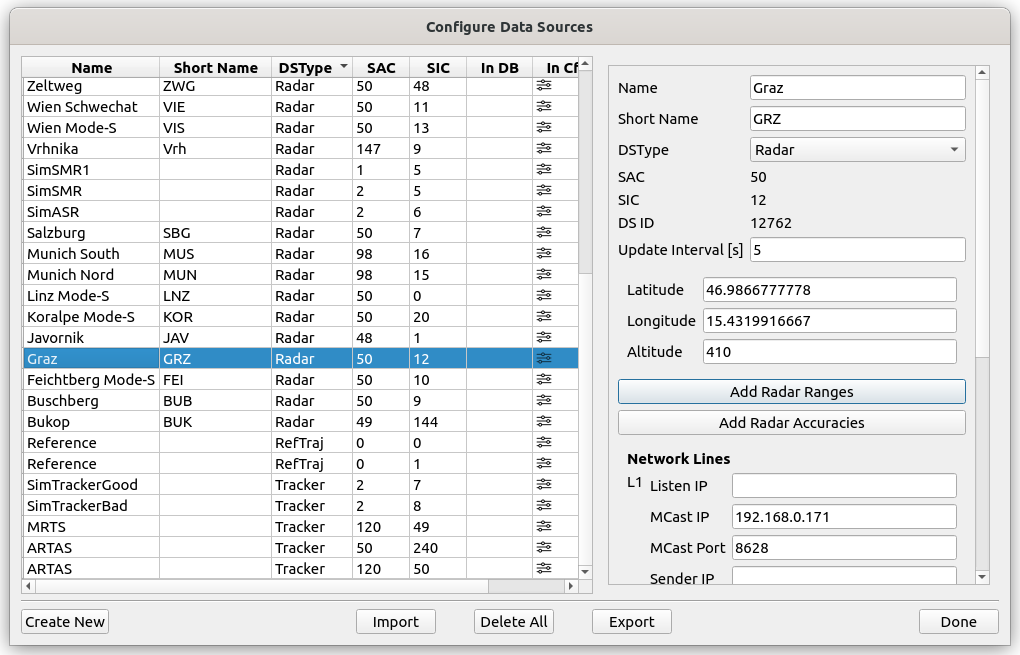
\includegraphics[width=18cm]{figures/configure_data_sources.png}
  \caption{Configure Data Sources}
\end{figure}

If data is imported from ASTERIX, data source information might be missing, so this information must either be edited manually, or loaded from a previous configuration (or a previous database containing the same information). \\

A data source is always stored in the configuration, which means it is persistent and can be used in all new databases. 
It is useful to define all existing data sources in the configuration, since they are immediately used during import of data. \\

A data source is stored in the database only if data from said source is imported. 
During the import, if a data source can be found (matching SAC/SIC) in the configuration, it is automatically added to the database. \\

Please \textbf{note} that currently the position of data sources is only required for \textbf{Radar} data sources (in the plot position calculation), for all other data sources it would suffice to have SAC/SIC and name information for display purposes. \\

However, for CAT010,CAT020 and CAT062 exists the option to project from a Cartesian X/Y coordinate system to WGS84 latitude and longitudes (when not available in the ASTERIX data). To use this feature during ASTERIX import, set a latitude/longitude for the respective data source.

\paragraph {Data Sources Table Content}
\label{sec:configure_datasources_table_content}

\begin{itemize}
\item Name: Name of the data source
\item Short Name: Short name of the data source (optional)
\item DSType: Data source type, e.g. Radar, MLAT, ADS-B, ...
\item SAC: System Area Code, number between [0,255]
\item SIC: System Identification Code, number between [0,255]
\item In DB: Indicator whether the data source is stored in the database
\item In Config: Indicator whether the data source is stored in the configuration
\end{itemize}
\ \\

When a data source is selected in the table, additional details are shown in the right side, where edting is also possible. \\

Please \textbf{note} that all changes to a data sources are always written to the database as well as the configuration. \\

Depending on the DSType, additional information can be set in a source. For a non-Radar source, the following information is given:

\begin{itemize}
\item ID: Number indentifier (unique)
\item Network Line information
\begin{itemize}
    \item 4 different lines are possible, each with 
    \begin{itemize}
      \item Listen IP (defines used network interface and IGMP requests, optional when not using multicast)
      \item Multicast IP
      \item Multicast port
      \item Sender IP (optional, for filtering purposes)
    \end{itemize}
\end{itemize}
\end{itemize}
\ \\

Please note that for using real multicast addressess (inside of 224.0.0.0 to 239.255.255.255), it is recommended to also define the Listen IP to the local address of the network interface to be used. Otherwise the multicast data might not be received, or the wrong network interface might be used, causing COMPASS to receive no data. \\

Please note that if e.g. only Multicast IP and port are set, and the Multicast IP is set to a non-multicast one (outside of 224.0.0.0 to 239.255.255.255), a local replay is possible (without real multi-casting). \\

For sources of DSType 'Radar', the follwing additional information should be provided:

\begin{itemize}
\item Latitude: Source center position as WGS-84 latitude, as floating point number in degrees, e.g. 42.0001
\item Longitude: Source center position as WGS-84 longitude, as floating point number in degrees, e.g. 17.01
\item Altitude: Source center altitude above MSL, in meters
\end{itemize}
\ \\

Additional optional information can be provided:

\subsubsection{Detection Type}

A detection type can be given of any data source, 'Mode S' is given as default. Currently only 'Primary Ground Only" used during reconstruction, but it is very important to set this type for SMRs, to mitigate sub-optimal association of primary-only target reports in close distances to clutter. \\

\begin{figure}[H]
  \center
    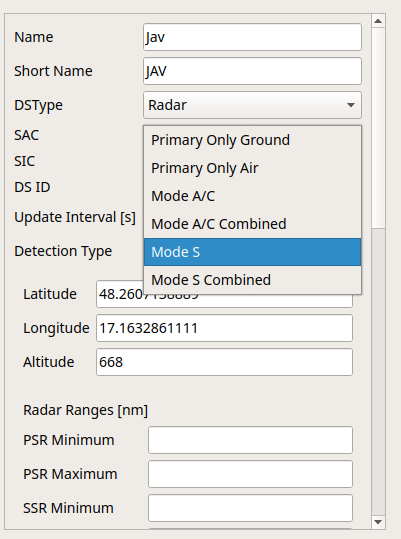
\includegraphics[width=8cm,frame]{figures/configure_ds_dettyp.png}
  \caption{Configure Data Sources: Detection type}
\end{figure}

\subsubsection{Radar Ranges \& Accuracies}

\begin{figure}[H]
  \center
    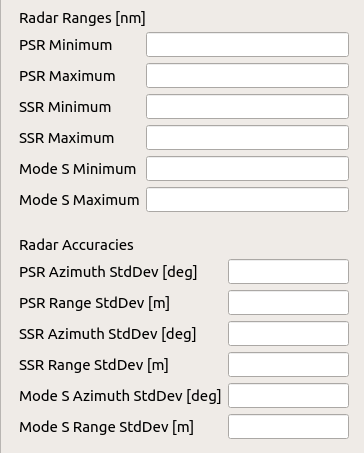
\includegraphics[width=8cm,frame]{figures/configure_data_sources_radar_details.png}
  \caption{Configure Data Sources: Radar details}
\end{figure}

\begin{itemize}
\item PSR Minimum: PSR minimum range, in nautical miles
\item PSR Maxmimum: PSR maximum range, in nautical miles
\item SSR Minimum: SSR minimum range, in nautical miles
\item SSR Maxmimum: SSR maximum range, in nautical miles
\item Mode S Minimum: Mode S minimum range, in nautical miles
\item Mode S Maxmimum: Mode S maximum range, in nautical miles
\item PSR Azimuth StdDev: PSR azimuth standard deviation, in degrees
\item PSR Range StdDev: PSR range standard deviation, in meters
\item SSR Azimuth StdDev: SSR azimuth standard deviation, in degrees
\item SSR Range StdDev: SSR range standard deviation, in meters
\item Mode S Azimuth StdDev: Mode S Radar azimuth standard deviation, in degrees
\item Mode S Range StdDev: Mode S Radar range standard deviation, in meters
\end{itemize}
\ \\

\subsubsection{Import/Export of Configuration Data Sources}
\label{sec:config_ds_export}

Using the 4 buttons on the bottom the following functions can be used:

\begin{itemize}
\item Create New: Create new data source
\item Import: Import configuration data sources from JSON file
\item Delete All: Delete all configuration data sources
\item Export: Export all configuration data sources as JSON file
\end{itemize}
\ \\

There are two versions of the data sources JSON file used for import/export. Please refer to \nameref{sec:appendix_data_sources}. \\

Using these functions, the configuration data sources can be changed for sensor context switches, or e.g. exported before an COMPASS version upgrade.
